%%%%%%%%%%%%%%%%%%%%%%%%%%%%%%%%%%%%%%%%%
% University/School Laboratory Report
% LaTeX Template
% Version 3.0 (4/2/13)
%
% This template has been downloaded from:
% http://www.LaTeXTemplates.com
%
% Original author:
% Linux and Unix Users Group at Virginia Tech Wiki 
% (https://vtluug.org/wiki/Example_LaTeX_chem_lab_report)
%
% License:
% CC BY-NC-SA 3.0 (http://creativecommons.org/licenses/by-nc-sa/3.0/)
%
%%%%%%%%%%%%%%%%%%%%%%%%%%%%%%%%%%%%%%%%%

%----------------------------------------------------------------------------------------
%	PACKAGES AND DOCUMENT CONFIGURATIONS
%----------------------------------------------------------------------------------------

\documentclass{article}

\usepackage[version=3]{mhchem} % Package for chemical equation typesetting
\usepackage{siunitx} % Provides the \SI{}{} command for typesetting SI units

\usepackage[top=1in, bottom=1in, right=1in, left=1in]{geometry}

%Add code formating
\usepackage{listings}
\lstset{tabsize=2}

\usepackage{hyperref}

\usepackage{amssymb}

\usepackage{enumerate}

%Add extra support for image placement
\usepackage{float}

\usepackage{mcode}

\usepackage{graphicx} % Required for the inclusion of images

\setlength\parindent{0pt} % Removes all indentation from paragraphs

\renewcommand{\labelenumi}{\alph{enumi}.} % Make numbering in the enumerate environment by letter rather than number (e.g. section 6)

% Setup how hyperlinks look
\usepackage{xcolor}
\hypersetup{
    colorlinks,
	linkcolor={red!50!black},
	citecolor={blue!50!black},
	urlcolor={blue!80!black},
}

%\usepackage{times} % Uncomment to use the Times New Roman font

%----------------------------------------------------------------------------------------
%	DOCUMENT INFORMATION
%----------------------------------------------------------------------------------------

\title{Keysight Hacking Platform Troubleshooting} % Title

\author{Blake \textsc{Vermeer}} % Author name

\date{\today} % Date for the report

\begin{document}

\maketitle % Insert the title, author and date

\begin{center}
\begin{tabular}{l r}
Date Performed: & April 13, 2017 \\ % Date the experiment was performed
Company: & Keysight Technologies % Company
\end{tabular}
\end{center}

% If you wish to include an abstract, uncomment the lines below
% \begin{abstract}
% Abstract text
% \end{abstract}

%----------------------------------------------------------------------------------------
%	OVERVIEW
%----------------------------------------------------------------------------------------
\section{Overview}

This document contains a list of common questions and their answers. You can use the contents menu in your PDF viewer to get a quick overview of the questions.


%----------------------------------------------------------------------------------------
%	User Accounts
%----------------------------------------------------------------------------------------
\section{What user accounts are set up on the Raspberry Pi?}

There are two user accounts set up on the Rasbperry Pi. There is a regular user account called \textit{keysight} and the administrator account called \textit{root}. The password for both accounts is \textbf{keysight}. Note - the sudo program is not installed in the image. If you need to create or edit any system files you will have to use the \textit{root} account. 

	\begin{table}[H]
	\centering
	
		\begin{tabular}[H]{| c | c |}
			\hline
			\textbf{User account} & \textbf{Password} \\
			\hline
			keysight & keysight \\
			\hline
			root & keysight \\
			\hline
		\end{tabular}
	
	\end{table}


%----------------------------------------------------------------------------------------
%	Change system settings
%----------------------------------------------------------------------------------------
\section{I need to change some system settings on the Raspberry Pi. How do I do that?}

You can do this by logging into a command shell on the Raspberry Pi by using the SSH protocol. On Linux and Mac systems the ssh program is installed by default. Simply start up a terminal emulator and type in \textbf{ssh \textless user account\textgreater @\textless device IP address\textgreater} (fill in the user account and IP address). You will then be prompted for the user account password. After entering the password you will be presented with a bash command prompt. \\

If you are using Windows you can download and install the \href{http://www.chiark.greenend.org.uk/~sgtatham/putty/latest.html}{PuTTY} program. PuTTY has an option in it to create an SSH connection to a device. After starting up the PuTTY program click the \textbf{SSH} option under connection type and enter the IP address of your Raspberry Pi in the \textbf{Host Name} box and then click open. You will then be prompted for the user account name to use and then the user password. After that you will be presented with a bash command prompt.

	\begin{figure}[H]
		\centering
		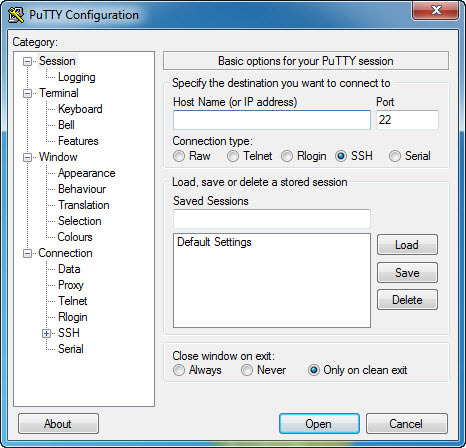
\includegraphics[width=0.5\textwidth]{pics/putty.jpg}
		\caption{PuTTY Program}
		\label{putty}
	\end{figure} 


%----------------------------------------------------------------------------------------
%	VM Slow
%----------------------------------------------------------------------------------------
\section{The VM image is running SLOW! Is there anything I can do about it?}

Besides upgrading your computer? ;-) Most modern CPU's support hardware virtualization acceleration. This feature greatly speeds up a virtual machine. But, some computer (especially business computers) ship with the AMD-V or Intel Vt-x feature disabled in the BIOS. Google your particular computer model or CPU model to find if your computer supports hardware virtulization. If it does and your VM is still run noticeably slow, it may be worth rebooting your computer into the BIOS and making sure either the AMD-V or Intel-Vt feature is enabled for your computer. 


%----------------------------------------------------------------------------------------
%	APPENDIX
%----------------------------------------------------------------------------------------

%\newpage
%\section{Appendix}

%\begin{enumerate}

	
%	\item[1. a.)] \lstinputlisting{../MATLAB/problem_1a.m}
	

%\end{enumerate}






%----------------------------------------------------------------------------------------


\end{document}